\documentclass[10pt,twocolumn, nofootinbib]{revtex4-1}
%\documentclass[aps,pra,10pt,twocolumn,floatfix,nofootinbib]{revtex4-1}
%\documentclass[10pt,twocolumn,letterpaper]{article}

\usepackage{amsmath}
\usepackage{amsfonts}
\usepackage{MnSymbol}
\usepackage{graphicx}
\usepackage{enumitem}
\usepackage{hyperref}
\hypersetup{
	colorlinks=true,
	citecolor=blue,
	urlcolor=blue,
	linkcolor=blue
}
\urlstyle{same}
\frenchspacing


\begin{document}

\title{Notes on classical/quantum logic }
\author{Gabriele Carcassi, Christine A. Aidala}
\affiliation{Physics Department, University of Michigan, Ann Arbor, MI 48109}

\date{\today}


\begin{abstract}
Notes of classical logic in quantum mechanics.
\end{abstract}

\maketitle

\section{Quantum logic: definition and motivation}

\subsection{Disjunction}

Connection between disjunction and superposition.

``A relevant feature of $\vee$ is that, differently from the case in classical semantics, a quantum disjunction may be true even if neither of it members is true. This reflects, for example, the case in which we are dealing with a state such as that of a spin 1/2 system which is in a linear combination of states up and down. Both propositions, ``the state is up'' and ``the state is down,'' may have no definite truth value (the excluded middle principle is violated), but the disjunction ``the state is up or the state is down'' is a tautology.''

\begin{description}
	\item $p =$ ``The particle has spin $z^+$''
	\item $q =$ ``The particle has spin $z^-$''
\end{description}

Claim: $p \vee q$ is \textbf{always} true, even if $p$ and $q$ may possibly be both false. The idea is that $p \vee q$ includes also all superpositions of $p$ and $q$.

Counterclaim. The propositions $p$ and $q$ are experimentally equivalent to:
\begin{description}
	\item $p =$ ``The expectation value for $S_z$ is 1/2$\hbar$''
	\item $q =$ ``The expectation value for $S_z$ is -1/2$\hbar$''
\end{description}
The proposition $p \vee q$ corresponds to the statement ``The absolute value of the expectation value for $S_z$ 1/2$\hbar$''. If we have a superposition of $p$ and $q$, the expectation value for $S_z$ will be strictly between $-1/2 \hbar$ and $1/2 \hbar$, and therefore $p \vee q$, when discussing expectation values, will be false as one would expect.

\subsection{Distributivity}

The distributivity in quantum mechanics is ``weird'' because (1) it can be true even if none of the elements of the disjunction is true due to the linearity of the Schroendinger equation and (2) quantum observables do not commute. 

\begin{description}
    \item $p =$ ``The particle has spin $x^+$''
    \item $q =$ ``The particle has spin $y^+$''
    \item $r =$ ``The particle has spin $y^-$''
\end{description}

Classic: $p \wedge (q \vee r)$ if and only if $(p \wedge  q) \vee (p \wedge r)$

Quantum: Assume $p$ is true, which means we measured spin $x$ to be $+$. Since if I measured spin $y$ I would either get $+$ or $-$, we have $q \vee r \equiv \top$. Therefore $q \vee r \equiv \top$ is true. On the other hand, both terms in the second disjunctions are false: because $p \wedge  q$ refer to incompatible observables, we have $p \wedge  q \equiv \bot$. Therefore the $(p \wedge  q) \vee (p \wedge r) \equiv \bot$.

$q \vee r \equiv \top$ therefore $p \wedge (q \vee r) \equiv p \wedge \top \equiv p$. If $p$ is true

\subsubsection{Reframing}

\begin{description}
    \item $p =$ ``The state of particle at time $t$ is $x^+$''
    \item $q =$ ``The state of particle at time $t$ is $y^+$''
    \item $r =$ ``The state of particle at time $t$ is $y^-$''
\end{description}

Then all three assertions are incompatible with each other. That is, $p \wedge q \equiv q \wedge r \equiv r \wedge p \equiv \bot$. Therefore $p \wedge (q \vee r) \equiv \bot \equiv (p \wedge  q) \vee (p \wedge r)$.

2 casi: considerare

\begin{description}
    \item $p =$ ``The state of particle at time $t$ is $x^+$''
    \item $q =$ ``The state of particle at time $t$ is $y^+$''
    \item $r =$ ``The state of particle at time $t$ is $y^-$''
    \item $\hat{q} =$ ``The state of particle at time $\hat{t}$ is $y^+$''
    \item $\hat{r} =$ ``The state of particle at time $\hat{t}$ is $y^-$''
\end{description}

In this case $p \wedge \hat{q} \nequiv \bot$ and $p \wedge \hat{r} \nequiv \bot$. Therefore the original claim was $p \wedge (\hat{q} \vee \hat{r})$ if and only if $(p \wedge  q) \vee (p \wedge r)$ which is not the classical logic distributive law. Note that, $\hat{q} \vee \hat{r} \equiv \top$ under condition that ``We measure spin $y$ at time $\hat{t}$''.

\subsubsection{Classical example}
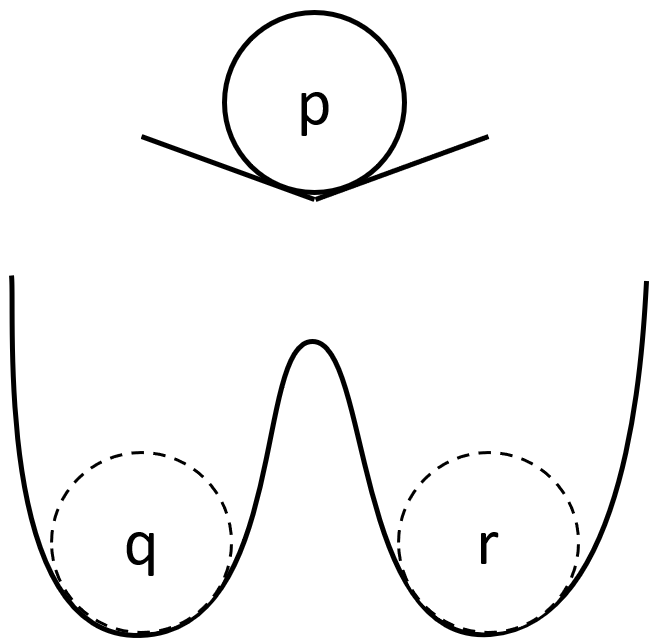
\includegraphics[width=\columnwidth]{Balldrop.png}

We have a ball sitting at position $p$ over a hatch. If the hatch opens, the ball drops, bounces around, until it will rest at either position $q$ or $r$ with equal chance. Two cases, as before:

\begin{description}
    \item $p =$ ``The position of the ball at time $t$ is $p$''
    \item $q =$ ``The position of the ball at time $t$ is $q$''
    \item $r =$ ``The position of the ball at time $t$ is $r$''
\end{description}

These are three incompatible assertions. Distributivity holds as before.

\begin{description}
    \item $p =$ ``The position of the ball at time $t$ is $p$''
    \item $q =$ ``The position of the ball at time $t$ is $q$''
    \item $r =$ ``The position of the ball at time $t$ is $r$''
    \item $\hat{q} =$ ``The position of the ball at time $\hat{t}$ is $q$''
    \item $\hat{r} =$ ``The position of the ball at time $\hat{t}$ is $r$''
\end{description}

We assume that, after time $t$, the hatch is opened and that at time $\hat{t}$ the ball has settled. As before, $\hat{q} \vee \hat{r} \equiv \top$ because the ball must be in one of the two positions after it dropped, therefore, if $p$ is true, the left side of the biconditional is true while the right side is false.

\section{Classical and quantum parallel}

Classical state: $\rho(x,p)$

Quantum state: $\psi(x)$

Classical observable $f(x,p)$. Average value $<f> = \int f(x, p) \rho(x, p) dx dp$. Eigenstate $f(x, p) \rho(x, p) = f_0 \rho(x, p)$.

Quantum observable $F$. Average value $<F> = \int \psi^\dagger(x) F \psi(x) dx$. Eigenstate $F \psi(x) = f_0 \psi(x)$.

In both cases, average value equal to $f_0$ means that the contributions of all parts of the ensemble combine to the value $f_0$. Eigenstate $f_0$ means all parts of the ensemble contribute the same value $f_0$.

For example, a classical eigenstate of $H = \frac{p^2}{2m} + \frac{1}{2} k x^2$ with eigenvalue $e_0$ is any function $\rho(x,p)$ that is different from zero only on the ellipses with energy $e_0$. That is, all elements of the distribution have the same energy.

The statement ``the observable $f$ of the system is between $f_0$ and $f_1$'' is therefore unclear. It could be taken to mean ``the average of observable $f$ of the system is between $f_0$ and $f_1$'' or ``the observable $f$ for each part of the ensemble is between $f_0$ and $f_1$''. In the first case, we are identifying a value from the real line, using the standard topology and the standard Borel algebra. In the second case, we are identifying a set of possible functions based on their support.

Now suppose that the $U$ and $V$ are two intervals. We have ``the average $<f>$ is in $U \cup V$'' is  equivalent to ``the average $<f>$ is in $U$'' $\vee$ ``the average $<f>$ is in $V$''. The average value must be in and and only one set. We also have ``the support of $\rho$ is $U \cup V$'' is not equivalent to ``the support of $\rho$ is $U$'' $\vee$ ``the support of $\rho$ is $V$''. The distribution could span both sets at the same time. But the lattice generated by such sets is still a $\sigma$-algebra, and therefore follows classical logic.

To check/prove: neither algebras is a sub-algebra of the other; both sub-algebras of the norm-induced one.

\section{Math}

* We can always use the Borel algebra for our statements. This will include(?) all propositions of ``quantum logic''.

It includes (?) also proposition on expectation values, say of position and momentum. Those will behave exactly like ``point particles''. It also includes (?) propositions on the support.

Show that this is similar to classical distributions.


Claim: in quantum mechanics the ``correct'' logical structure the is algebra of subspaces of the Hilbert space. In this algebra (which is a $\cap$-structure) the meet functions differently than in Boolean logic. Therefore it does not follow classical logic.

Resolution: that algebra does not include many statements that are interesting experimentally. For example, it does not include statements about the expectation values which, in the end, are the result of experiments. (Cross-section?) One 


Technical view: the state space of quantum states is a separable Hilbert space; it is a Banach space (complete normed space) and admits a norm-induced topology; it is separable, so it admits a countable basis, so the topology is second countable; therefore the state space has a countably generated Borel-algebra. This, like any set theoretic structure, follows Boolean algebra. Each state is a point and state-statements like ``the system is in state $s_1$'' are singletons in the $\sigma$-algebra. State-statements are all incompatible with each other: either we prepared one state or we prepared another.

If a process with an initial and final state (the internal are disregarded), we have two lattices of propositions. The sample space is the Cartesian product, the $\sigma$-algebra is the product. A measurement process will follow this pattern. We can say ``the system was prepared in state $s$'' and ``the system was measure in state $s$'' and there are two different statements. In the product algebra, we can then mix and match statements with the usual Boolean constructs. Both these are analogous in a classical and quantum case. These will naturally result in different lattices, but they will still be Boolean lattices.

What changes are the probability spaces we can construct. In the quantum case, the probability is not in general a probability measure and has to be consistent with the Born rule (i.e. the inner product).


\bibliography{quantumlogic}


\end{document}
